\chapter{Appendix}\label{chapter:Appendix}

\section{Results Data Leakage}
\sisetup{
  table-format = 1.4,    % maximal 1 Vorkommastelle, 4 Nachkommastellen
  detect-all            % übernimmt Schriftart/Fettdruck
}

% ---------- eigene Spaltentypen ----------
\newcolumntype{d}{S}     % „d“ steht für Dezimalspalte

\begin{table}[htbp]
\centering
\caption{OpenAI GPT-4o: Data Leakage (DL) based on 3 iterations}
\small                 % optional verkleinern
\setlength{\tabcolsep}{6pt} % enger packen, falls nötig
\begin{tabular}{
  l               % Model
  l               % Prompt
  | d        % Full Page (3 Spalten)
  | d d d d d     % Interaction Part (5 Spalten)
}
\toprule
\cmidrule(lr){3-3}\cmidrule(l){4-8}
\multicolumn{2}{c|}{\textbf{}} & {\bfseries Final Score} & {Size} & {Text} & {Position} & {Text Color} & {CLIP}\\
\midrule
% ---------------- Modell 1 ----------------
\multirow{4}{*}{DL Test Dataset} 
  & Naive & \bfseries 0.8917 & 0.8812 & 0.9701 & 0.8562 & 0.8451 & 0.906\\
  & Zero-Shot    & \bfseries 0.8889 & 0.866 & 0.9737 & 0.8543 & 0.8407 & 0.9098\\
  & Few-Shot   & \bfseries 0.8929 & 0.8929 & 0.9756 & 0.8486 & 0.8394 & 0.9078\\
  & Reasoning & \bfseries 0.8924 & 0.8819 & 0.9755 & 0.8498 & 0.8449 & 0.91\\
  & Iterative & \bfseries 0.8908 & 0.8819 & 0.9748 & 0.8475 & 0.8391 & 0.9109\\
  & Iterative Refine 1 & \bfseries 0.8878 & 0.8729 & 0.974 & 0.8469 & 0.8372 & 0.9081\\
  & Iterative Refine 2 & \bfseries 0.8887 & 0.8642 & 0.9771 & 0.8516 & 0.8439 & 0.9069\\
  & Iterative Refine 3 & \bfseries 0.8871 & 0.8497 & 0.979 & 0.8511 & 0.8483 & 0.9076\\
\midrule
% ---------------- Modell 2 ----------------
\multirow{4}{*}{Experiment Dataset}
  & Naive & \bfseries 0.8896 & 0.868 & 0.9661 & 0.8578 & 0.8456 & 0.9107\\
  & Zero-Shot    & \bfseries 0.8779 & 0.8124 & 0.9663 & 0.8558 & 0.8467 & 0.9083\\
  & Few-Shot   & \bfseries 0.8729 & 0.8131 & 0.9645 & 0.8562 & 0.8242 & 0.9067\\
  & Reasoning & \bfseries 0.8791 & 0.8348 & 0.9652 & 0.8549 & 0.8358 & 0.9048\\
  & Iterative & \bfseries 0.8854 & 0.8447 & 0.9694 & 0.8577 & 0.8412 & 0.914\\
  & Iterative Refine 1 & \bfseries 0.8786 & 0.8306 & 0.9677 & 0.858 & 0.8233 & 0.9131\\
  & Iterative Refine 2 & \bfseries 0.8767 & 0.8148 & 0.968 & 0.854 & 0.8315 & 0.915\\
  & Iterative Refine 3 & \bfseries 0.8731 & 0.811 & 0.9685 & 0.855 & 0.8181 & 0.9127\\
\midrule
% ---------------- weitere Modelle hier ----------------
% (dupliziere das obige Muster)
\bottomrule
\end{tabular}
\end{table}

\begin{table}[htbp]
\centering
\caption{Gemini-2.0-flash: Data Leakage (DL) based on 3 iterations}
\small                 % optional verkleinern
\setlength{\tabcolsep}{6pt} % enger packen, falls nötig
\begin{tabular}{
  l               % Model
  l               % Prompt
  | d        % Full Page (3 Spalten)
  | d d d d d     % Interaction Part (5 Spalten)
}
\toprule
\cmidrule(lr){3-3}\cmidrule(l){4-8}
\multicolumn{2}{c|}{\textbf{}} & {\bfseries Final Score} & {Size} & {Text} & {Position} & {Text Color} & {CLIP}\\
\midrule
% ---------------- Modell 1 ----------------
\multirow{4}{*}{DL Test Dataset} 
  & Naive & \bfseries 0.8801 & 0.7992 & 0.9685 & 0.8591 & 0.8251 & 0.9079\\
  & Zero-Shot    & \bfseries 0.8798 & 0.8297 & 0.977 & 0.8645 & 0.8141 & 0.9134\\
  & Few-Shot   & \bfseries 0.8729 &  0.8131 &  0.9645 &  0.8562 &  0.8242 &  0.9067\\
  & Reasoning & \bfseries 0.8683 & 0.799 & 0.9741 & 0.8541 & 0.8093 & 0.905\\
  & Iterative & \bfseries 0.8823 & 0.8298 & 0.9742 & 0.8624 & 0.836 & 0.9091\\
  & Iterative Refine 1 & \bfseries 0.8783 & 0.8297 & 0.9753 & 0.8616 & 0.8136 & 0.9112\\
  & Iterative Refine 2 & \bfseries 0.8874 & 0.8617 & 0.9774 & 0.871 & 0.8182 & 0.9086\\
  & Iterative Refine 3 & \bfseries 0.8899 & 0.8682 & 0.9773 & 0.8719 & 0.8224 & 0.9099\\
\midrule
% ---------------- Modell 2 ----------------
\multirow{4}{*}{Experiment Dataset}
  & Naive & \bfseries 0.8712 & 0.7992 & 0.9686 & 0.8591 & 0.8215 & 0.9079\\
  & Zero-Shot    & \bfseries 0.8685 & 0.7875 & 0.9687 & 0.862 & 0.8166 & 0.9094\\
  & Few-Shot   & \bfseries  0.8695 & 0.7989 & 0.9658 & 0.8627 & 0.8154 & 0.9048\\
  & Reasoning & \bfseries 0.868 & 0.7916 & 0.963 & 0.8594 & 0.7996 & 0.9067\\
  & Iterative & \bfseries 0.8707 & 0.7891 & 0.9686 & 0.8657 & 0.8209 & 0.9093\\
  & Iterative Refine 1 & \bfseries 0.8622 & 0.7703 & 0.9654 & 0.8616 & 0.8073 & 0.9064\\
  & Iterative Refine 2 & \bfseries 0.8676 & 0.7803 & 0.9683 & 0.8724 & 0.8132 & 0.9039\\
  & Iterative Refine 3 & \bfseries 0.8609 & 0.7708 & 0.9672 & 0.8707 & 0.7939 & 0.9017\\
\midrule
% ---------------- weitere Modelle hier ----------------
% (dupliziere das obige Muster)
\bottomrule
\end{tabular}
\end{table}






\newpage





\section{Results Code Similarity}
\sisetup{
  table-format = 1.4,  
  detect-all       
}


\newcolumntype{d}{S} 

\begin{table}[htbp]
\centering
\caption{Results of Code Similarity for each model based on 3 runs.}
\small  
\setlength{\tabcolsep}{6pt}
\begin{tabular}{
  l   
  l   
  | d  
  | d d d d d 
}
\toprule
\cmidrule(lr){3-3}\cmidrule(l){4-8}
\multicolumn{2}{c|}{\textbf{}} & {\bfseries Final Score} & {Size} & {Text} & {Position} & {Text Color} & {CLIP}\\
\midrule

\multirow{4}{*}{Gemini} 
  & Naive & \bfseries 0.8712 & 0.7992 & 0.9686 & 0.8591 & 0.8215 & 0.9079\\
  & Zero-Shot    & \bfseries 0.8685 & 0.7875 & 0.9687 & 0.862 & 0.8166 & 0.9094\\
  & Few-Shot   & \bfseries  0.8695 & 0.7989 & 0.9658 & 0.8627 & 0.8154 & 0.9048\\
  & Chain-of-Thought & \bfseries 0.868 & 0.7916 & 0.963 & 0.8594 & 0.7996 & 0.9067\\
  & Iterative Refine 1 & \bfseries 0.8622 & 0.7703 & 0.9654 & 0.8616 & 0.8073 & 0.9064\\
  & Iterative Refine 2 & \bfseries 0.8676 & 0.7803 & 0.9683 & 0.8724 & 0.8132 & 0.9039\\
  & Iterative Refine 3 & \bfseries 0.8609 & 0.7708 & 0.9672 & 0.8707 & 0.7939 & 0.9017\\
  & Composite & \bfseries 0.8559 & 0.774 & 0.9656 & 0.8596 & 0.7744 & 0.9059\\
  & Agent & \bfseries 0.8507 & 0.7509 & 0.9631 & 0.8489 & 0.7901 & 0.9004\\
\midrule

\multirow{4}{*}{ChatGPT}
  & Naive & \bfseries 0.8896 & 0.868 & 0.9661 & 0.8578 & 0.8456 & 0.9107\\
  & Zero-Shot    & \bfseries 0.8779 & 0.8124 & 0.9663 & 0.8558 & 0.8467 & 0.9083\\
  & Few-Shot   & \bfseries 0.8729 & 0.8131 & 0.9645 & 0.8562 & 0.8242 & 0.9067\\
  & Chain-of-Thought & \bfseries 0.8791 & 0.8348 & 0.9652 & 0.8549 & 0.8358 & 0.9048\\
  & Iterative Refine 1 & \bfseries 0.8786 & 0.8306 & 0.9677 & 0.858 & 0.8233 & 0.9131\\
  & Iterative Refine 2 & \bfseries 0.8767 & 0.8148 & 0.968 & 0.854 & 0.8315 & 0.915\\
  & Iterative Refine 3 & \bfseries 0.8731 & 0.811 & 0.9685 & 0.855 & 0.8181 & 0.9127\\
  & Composite & \bfseries 0.8642 & 0.8061 & 0.9666 & 0.853 & 0.7879 & 0.9072\\
  & Agent & \bfseries 0.8612 & 0.781 & 0.9631 & 0.8456 & 0.8081 & 0.9081\\
\midrule

\multirow{4}{*}{Qwen}
  & Naive & \bfseries 0.7036 & 0.6336 & 0.7755 & 0.6348 & 0.6313 & 0.8427\\
  & Zero-Shot    & \bfseries 0.6875 & 0.63 & 0.7561 & 0.6105 & 0.6032 & 0.8377\\
  & Few-Shot   & \bfseries 0.747 & 0.6813 & 0.8507 & 0.6809 & 0.6601 & 0.8619\\
  & Chain-of-Thought & \bfseries 0.8194 & 0.7557 & 0.9545 & 0.7748 & 0.7454 & 0.8668\\
  & Iterative Refine 1 & \bfseries 0.7083 & 0.6081 & 0.7976 & 0.6422 & 0.6451 & 0.8484\\
  & Iterative Refine 2 & \bfseries 0.7006 & 0.5926 & 0.7896 & 0.6369 & 0.637 & 0.8467\\
  & Iterative Refine 3 & \bfseries 0.7046 & 0.584 & 0.7985 & 0.6451 & 0.6459 & 0.8494\\
  & Composite & \bfseries 0.7147 & 0.6371 & 0.7985 & 0.644 & 0.6468 & 0.8472\\
  & Agent & \bfseries 0.7101 & 0.6305 & 0.7873 & 0.6423 & 0.6462 & 0.8439\\
\midrule

\bottomrule
\end{tabular}
\end{table}






\newpage





\sisetup{
  detect-all,
  table-format = 4.0        % up to 4‑digit integer
}

% ----------------------------------------------------------------
\begin{table}[htbp]
  \centering
  \scriptsize                             % <- tweak size here
  \caption{Accessibility violations (absolute and mean per file)
           across prompting techniques and models.}
  \setlength{\tabcolsep}{6pt}
  \begin{tabular}{l l S S[table-format=1.2]}
    \toprule
    \multicolumn{2}{c}{\textbf{}} &
      \textbf{\# Viol.} &
      \textbf{Mean/file} \\
    \midrule

    % ---------- Gemini ----------
    \multirow{9}{*}{Gemini}
      & Naive                &  432 & 2.10 \\
      & Zero‑Shot            &  451 & 2.19 \\
      & Few‑Shot             &  428 & 2.07 \\
      & Chain‑of‑Thought     &  439 & 2.12 \\
      & IterativeRef1     &  415 & 2.01 \\
      & IterativeRef2     &  408 & 1.98 \\
      & IterativeRef3     &  421 & 2.05 \\
      & Composite            &  399 & 1.93 \\
      & Agent                &  387 & 1.88 \\
    \midrule

    % ---------- ChatGPT ----------
    \multirow{9}{*}{ChatGPT}
      & Naive                &  378 & 1.84 \\
      & Zero‑Shot            &  395 & 1.92 \\
      & Few‑Shot             &  369 & 1.80 \\
      & Chain‑of‑Thought     &  382 & 1.86 \\
      & IterativeRef1     &  359 & 1.75 \\
      & IterativeRef2     &  351 & 1.72 \\
      & IterativeRef3     &  364 & 1.78 \\
      & Composite            &  346 & 1.68 \\
      & Agent                &  341 & 1.66 \\
    \midrule

    % ---------- Qwen ----------
    \multirow{9}{*}{Qwen}
      & Naive                &  612 & 3.04 \\
      & Zero‑Shot            &  598 & 2.97 \\
      & Few‑Shot             &  572 & 2.85 \\
      & Chain‑of‑Thought     &  529 & 2.64 \\
      & IterativeRef1     &  601 & 3.00 \\
      & IterativeRef2     &  609 & 3.05 \\
      & IterativeRef3     &  595 & 2.98 \\
      & Composite            &  583 & 2.92 \\
      & Agent                &  589 & 2.95 \\
    \bottomrule
  \end{tabular}
\end{table}


  




\newpage





\lstset{
  language=HTML,
  basicstyle=\ttfamily\scriptsize,
  numbers=left,
  frame=single
}

\begin{figure}
  \centering
  \begin{subfigure}[t]{0.46\textwidth}
    \adjustbox{valign=t}{%
      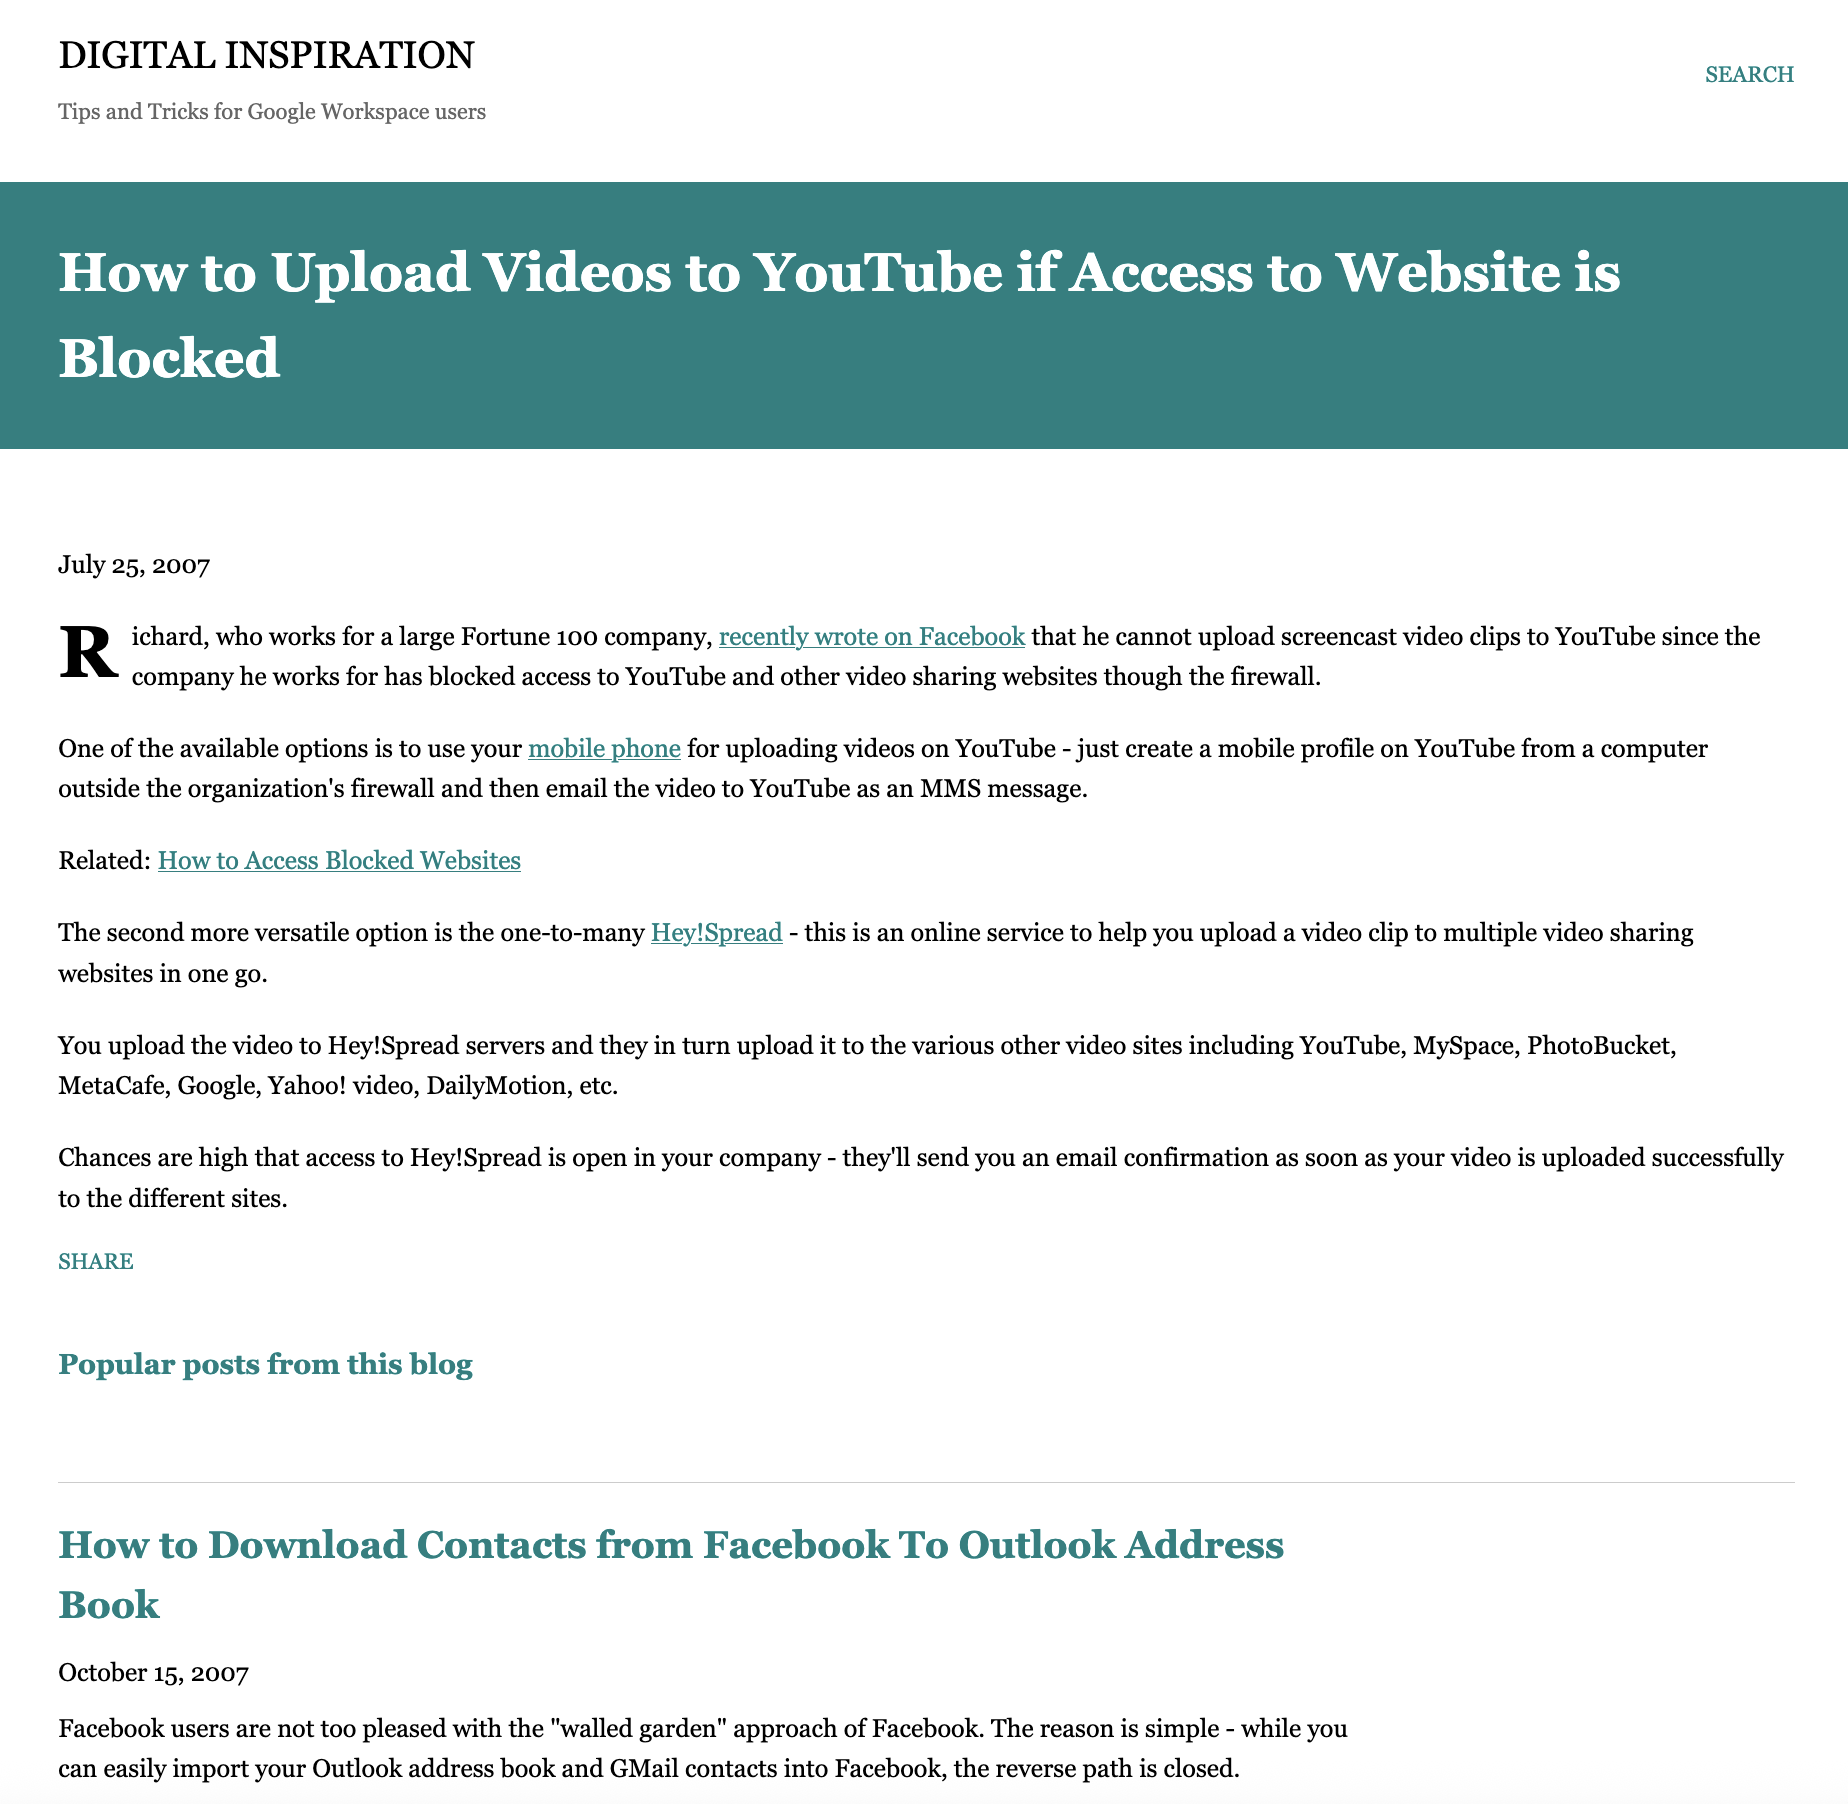
\includegraphics[width=\linewidth]{figures/landmarkwebpageexample.png}}
    \caption{Rendered webpage used as input}
    \label{fig:webpage}
  \end{subfigure}\hfill
  \begin{subfigure}[t]{0.48\textwidth}
    \vspace{0pt}%
    \begin{lstlisting}
<!-- generated by ChatGPT-4o -->
<!DOCTYPE html>
<html lang="en">
  <head> ... </head>

  <body>
    <div class="header"> ... </div>
    <div class="title-section"> ... </div>
    <div class="main-content"> ... </div>
    <div class="footer"> ... </div>
  </body>
</html>
    \end{lstlisting}
    \caption{HTML output from Model ChatGPT-4o lacking semantic landmarks}
    \label{lst:html}
  \end{subfigure}
  \caption{ChatGPT-4o accurately reproduces the visual layout shown in (a), yet omits semantic landmark elements, such as \texttt{<header>} and \texttt{<main>} in the generated HTML (b)}
  \label{fig:landmarkcomparison}
\end{figure}









\newpage








\begin{figure}[htbp]
  \centering
  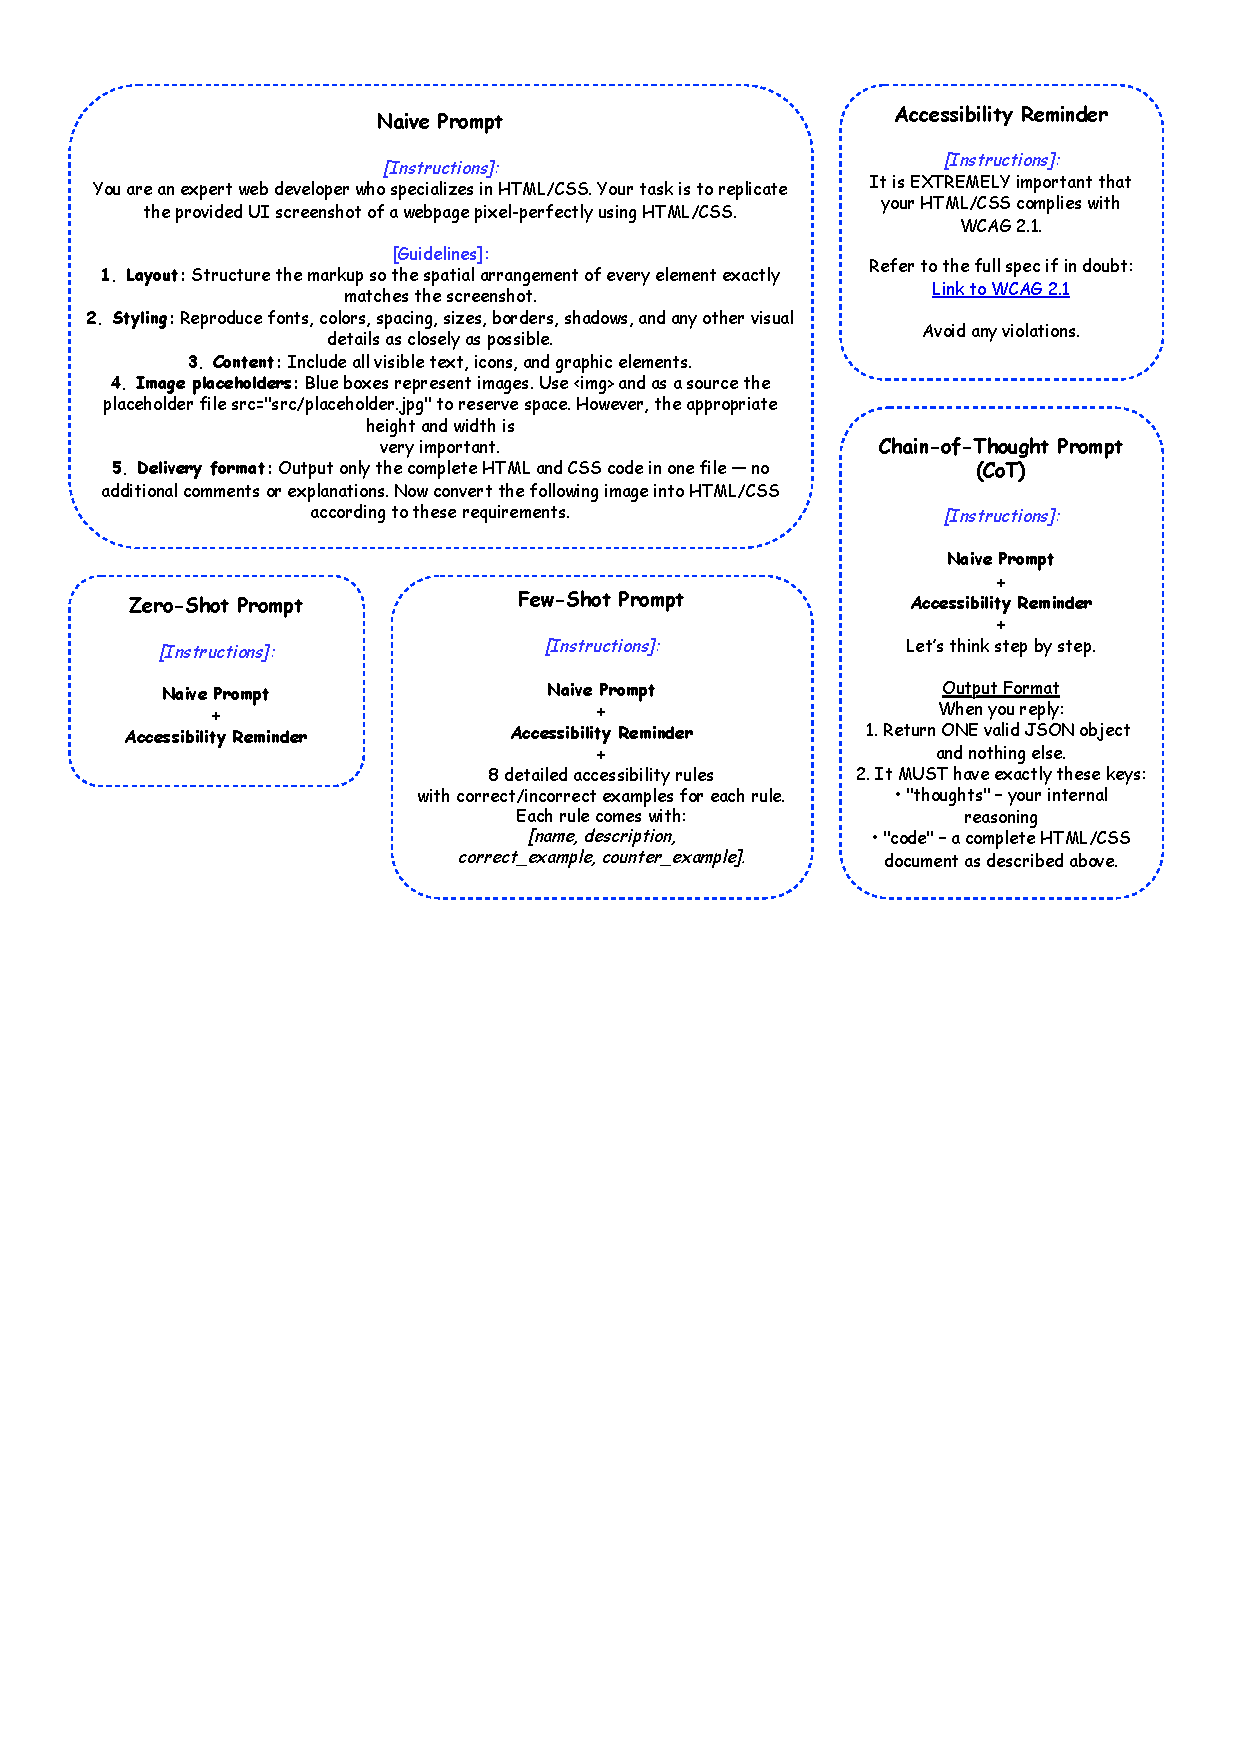
\includegraphics[page=1,width=\linewidth,trim=0cm 14cm 0cm 0cm,clip,]{figures/prompts.pdf}
  \caption{Overview of Prompts used.}
  \label{fig:prompt-overview}
\end{figure}







\newpage








% \section{Accessibility Violations Resolved}
% \pgfplotsset{compat=1.18}                    % aktuelle Syntax

% % ---------------- Farben definieren ---------------------
% \definecolor{usable}{RGB}{ 54, 95,230}   % kräftiges Blau
% \definecolor{unusable}{RGB}{234,127,111} % rötlicher Ton

% \begin{tikzpicture}
% \begin{axis}[
%   % --- Achsen-/Diagramm-Eigenschaften -------------------
%   xbar stacked,                 % horizontale, gestapelte Balken
%   xmin=0, xmax=100,             % 0–100 %
%   width=13cm, height=12cm,      % Gesamtgröße
%   bar width=8pt,                % Balkendicke
%   enlarge y limits=0.05,        % etwas Luft oben/unten
%   xlabel={Percentage (\%)},
%   axis x line*=bottom,          % nur untere x-Achse
%   axis y line*=left,            % nur linke y-Achse
%   ytick=data,                   % ein Tick pro Kategorie
%   y tick label style={font=\small},
%   % --- Legende oben -------------------------------------
%   legend style={
%     at={(0.5,1.06)}, anchor=south, draw=none,
%     legend cell align=left, font=\small
%   },
%   % --- Werte im Balken (nur im 1. Plot) -----------------
%   nodes near coords,
%   nodes near coords style={
%     font=\scriptsize\bfseries, text=white, anchor=center
%   },
%   every node near coord/.append style={
%     /pgf/number format/.cd, fixed, precision=0,  % nur ganze %
%     /tikz/.cd
%   },
%   % --- Kategorien (y-Achse) in genau der Reihenfolge ----
%   symbolic y coords={
%     Claude (Mark), Claude (CoT), Claude (Direct),
%     GPT-4o (Mark), GPT-4o (CoT), GPT-4o (Direct),
%     Gemini (Mark), Gemini (CoT), Gemini (Direct),
%     Qwen-72B (Mark), Qwen-72B (CoT), Qwen-72B (Direct),
%     Qwen-7B (Mark), Qwen-7B (CoT), Qwen-7B (Direct),
%     Qwen-3B (Mark), Qwen-3B (CoT), Qwen-3B (Direct)
%   }
% ]
% % ---------- 1. Plot: Usable (blau) + Prozentzahlen -------
% % ---------- 1. Plot: Usable -----------------------------
% \addplot+[xbar,fill=usable] coordinates {
%   (77,{Claude (Mark)})   (69,{Claude (CoT)})   (66,{Claude (Direct)})
%   (81,{GPT-4o (Mark)})   (74,{GPT-4o (CoT)})   (73,{GPT-4o (Direct)})
%   (64,{Gemini (Mark)})   (53,{Gemini (CoT)})   (47,{Gemini (Direct)})
%   (54,{Qwen-72B (Mark)}) (43,{Qwen-72B (CoT)}) (41,{Qwen-72B (Direct)})
%   (32,{Qwen-7B (Mark)})  (22,{Qwen-7B (CoT)})  (30,{Qwen-7B (Direct)})
%   (18,{Qwen-3B (Mark)})  (19,{Qwen-3B (CoT)})  (17,{Qwen-3B (Direct)})
% };

% % ---------- 2. Plot: Unusable ---------------------------
% \addplot+[xbar,fill=unusable,nodes near coords={}] coordinates {
%   (23,{Claude (Mark)})   (31,{Claude (CoT)})   (34,{Claude (Direct)})
%   (19,{GPT-4o (Mark)})   (26,{GPT-4o (CoT)})   (27,{GPT-4o (Direct)})
%   (36,{Gemini (Mark)})   (47,{Gemini (CoT)})   (53,{Gemini (Direct)})
%   (46,{Qwen-72B (Mark)}) (57,{Qwen-72B (CoT)}) (59,{Qwen-72B (Direct)})
%   (68,{Qwen-7B (Mark)})  (78,{Qwen-7B (CoT)})  (70,{Qwen-7B (Direct)})
%   (82,{Qwen-3B (Mark)})  (81,{Qwen-3B (CoT)})  (83,{Qwen-3B (Direct)})
% };

% \legend{Usable, Unusable}
% \end{axis}
% \end{tikzpicture}






\newpage







\newcolumntype{L}[1]{>{\raggedright\arraybackslash}p{#1}}
\newcolumntype{Y}{>{\raggedright\arraybackslash}X}

\begin{table}[htbp]
\footnotesize                        % ggf. \scriptsize, wenn sehr viel Inhalt
\setlength{\tabcolsep}{3pt}          % enger setzen
\caption{Mapped Accessibility-Violations}\label{tab:a11y-onepage}
\begin{tabularx}{\textwidth}{|L{2cm}|L{4.5cm}|L{3.5cm}|Y|}
\hline
\textbf{Technique} & \textbf{Success Criterion} &
\textbf{Mapping-Name} & \textbf{Description}\\ \hline

\href{https://www.w3.org/TR/WCAG20-TECHS/H30.html}{H30.2},
\href{https://www.w3.org/TR/WCAG20-TECHS/H91.html}{H91.A} &
\href{https://dequeuniversity.com/rules/axe/4.10/link-name}{link-name} &
Links; Missing descriptive content of \texttt{<a>} &
Link has no perceivable (visible/AT) name.\\ \hline

-- &
\href{https://dequeuniversity.com/rules/axe/4.10/link-in-text-block}{link-in-text-block} &
Links; Distinguishable Color &
Only color distinguishes the link from body text.\\ \hline


\href{https://www.w3.org/TR/WCAG20-TECHS/H59.html}{H59} &
-- &
Links; Uncomplete &
Incomplete or malformed \texttt{<a>} element.\\ \hline


\href{https://www.w3.org/TR/WCAG20-TECHS/H36.html}{H36},
\href{https://www.w3.org/TR/WCAG20-TECHS/H37.html}{H37},
\href{https://www.w3.org/TR/WCAG20-TECHS/H67.html}{H67} &
\href{https://dequeuniversity.com/rules/axe/4.10/image-alt}{image-alt},
\href{https://dequeuniversity.com/rules/axe/4.10/input-image-alt}{input-image-alt} &
Alt‑Text; Images &
Image lacks alternative text.\\ \hline


\href{https://www.w3.org/TR/WCAG20-TECHS/H2.html}{H2} &
\href{https://dequeuniversity.com/rules/axe/4.10/image-redundant-alt}{image-redundant-alt} &
Alt‑Text; Images and Links; Redundant Alt‑Text &
Alt text simply repeats visible text.\\ \hline


\href{https://www.w3.org/TR/WCAG20-TECHS/H42.html}{H42},
\href{https://www.w3.org/TR/WCAG20-TECHS/G141.html}{G141} &
\href{https://dequeuniversity.com/rules/axe/4.10/page-has-heading-one}{page-has-heading-one},
\href{https://dequeuniversity.com/rules/axe/4.10/heading-order}{heading-order},
\href{https://dequeuniversity.com/rules/axe/4.10/empty-heading}{empty-heading} &
Headings; Wrong Order, Empty and Missing Headings; &
Headings missing, empty, or out of logical order.\\ \hline

-- &
\href{https://dequeuniversity.com/rules/axe/4.10/landmark-one-main}{landmark-one-main},
\href{https://dequeuniversity.com/rules/axe/4.10/landmark-unique}{landmark-unique},
\href{https://dequeuniversity.com/rules/axe/4.10/region}{region},
\href{https://dequeuniversity.com/rules/axe/4.10/landmark-no-duplicate-contentinfo}{landmark-no-duplicate-contentinfo},
\href{https://dequeuniversity.com/rules/axe/4.10/landmark-no-duplicate-main}{landmark-no-duplicate-main},
\href{https://dequeuniversity.com/rules/axe/4.10/landmark-main-is-top-level}{landmark-main-is-top-level} &
Landmark and Region; Missing and Unique Landmarks; &
Landmarks missing, duplicated, or incorrectly nested.\\ \hline


\href{https://www.w3.org/TR/WCAG20-TECHS/H91.html}{H91},
\href{https://www.w3.org/TR/WCAG20-TECHS/F68.html}{F68} &
\href{https://dequeuniversity.com/rules/axe/4.10/label}{label} &
Label; Multiple Elements; Content missing &
Form controls missing or having multiple labels/content.\\ \hline


\href{https://www.w3.org/TR/WCAG20-TECHS/H91.html}{H91}&
\href{https://dequeuniversity.com/rules/axe/4.10/input-button-name}{input-button-name},
\href{https://dequeuniversity.com/rules/axe/4.10/button-name}{button-name} &
Label; Button; Missing Label &
(Button) control lacks an accessible name.\\ \hline

\href{https://www.w3.org/TR/WCAG20-TECHS/H93.html}{H93},
\href{https://www.w3.org/TR/WCAG20-TECHS/H44.html}{H44},
\href{https://www.w3.org/TR/WCAG20-TECHS/H65.html}{H65} &
\href{https://dequeuniversity.com/rules/axe/4.10/form-field-multiple-labels}{form-field-multiple-labels} &
Label; Form Field; Multiple IDs, No ID, Wrong for attribute &
Form field with multiple/incorrect labels or IDs.\\ \hline


\href{https://www.w3.org/TR/WCAG20-TECHS/H63.html}{H63}&
\href{https://dequeuniversity.com/rules/axe/4.10/scope-attr-valid}{scope-attr-valid},
\href{https://dequeuniversity.com/rules/axe/4.10/td-headers-attr}{td-headers-attr} &
Tables; Scope Attribute; &
Incorrect scope/headers association in table.\\ \hline


\href{https://www.w3.org/TR/WCAG20-TECHS/H43.html}{H43},
\href{https://www.w3.org/TR/WCAG20-TECHS/H63.html}{H63} &
\href{https://dequeuniversity.com/rules/axe/4.10/empty-table-header}{empty-table-header} &
Tables; Table Headers; &
Table headers missing, empty, or wrongly referenced.\\ \hline


-- &
\href{https://dequeuniversity.com/rules/axe/4.10/td-has-header}{td-has-header} &
Tables; Table Data must have Table Header; &
Data cells missing an associated header.\\ \hline


\href{https://www.w3.org/TR/WCAG20-TECHS/G18.html}{G18},
\href{https://www.w3.org/TR/WCAG20-TECHS/G145.html}{G145},
\href{https://www.w3.org/TR/WCAG20-TECHS/G17.html}{G17} &
\href{https://dequeuniversity.com/rules/axe/4.10/color-contrast}{color-contrast},
\href{https://dequeuniversity.com/rules/axe/4.10/color-contrast-enhanced}{color-contrast-enhanced} &
Color Contrast; Text; &
Insufficient text/background contrast.\\ \hline


\href{https://www.w3.org/TR/WCAG20-TECHS/H25.html}{H25.1} &
\href{https://dequeuniversity.com/rules/axe/4.10/document-title}{document-title} &
Title; Document Title; &
Document title missing or empty.\\ \hline


\href{https://www.w3.org/TR/WCAG20-TECHS/H57.html}{H57},
\href{https://www.w3.org/TR/WCAG20-TECHS/H58.html}{H58.1} &
\href{https://dequeuniversity.com/rules/axe/4.10/html-has-lang}{html-has-lang},
\href{https://dequeuniversity.com/rules/axe/4.10/html-lang-valid}{html-lang-valid},
\href{https://dequeuniversity.com/rules/axe/4.10/html-xml-lang-mismatch}{html-xml-lang-mismatch},
\href{https://dequeuniversity.com/rules/axe/4.10/valid-lang}{valid-lang} &
Language; Document Lang; Missing and Invalid &
HTML language missing or invalid.\\ \hline


\href{https://www.w3.org/TR/WCAG20-TECHS/H32.html}{H32} &
-- &
Elements; Form; No Submit Button &
Form lacks a submit mechanism.\\ \hline


\href{https://www.w3.org/TR/WCAG20-TECHS/F77.html}{F77} &
-- &
ID; Duplicate IDs; &
Duplicate \texttt{id} attributes.\\ \hline


-- &
\href{https://dequeuniversity.com/rules/axe/4.10/target-size}{target-size} &
Size; Target Size; Element too small &
Interactive target too small.\\ \hline


-- &
\href{https://dequeuniversity.com/rules/axe/4.10/aria-prohibited-attr}{aria-prohibited-attr} &
Aria Attributes; Prohibited Attributes; &
Prohibited ARIA attribute used.\\ \hline


-- &
\href{https://dequeuniversity.com/rules/axe/4.10/aria-valid-attr-value}{aria-valid-attr-value},
\href{https://dequeuniversity.com/rules/axe/4.10/aria-valid-attr}{aria-valid-attr} &
Aria Attributes; Valid Values; &
Invalid ARIA attribute value.\\ \hline


-- &
\href{https://dequeuniversity.com/rules/axe/4.10/aria-allowed-attr}{aria-allowed-attr} &
Aria Attributes; Allowed Attributes; &
ARIA attribute not permitted for role.\\ \hline


-- &
\href{https://dequeuniversity.com/rules/axe/4.10/label-title-only}{label-title-only},
\href{https://dequeuniversity.com/rules/axe/4.10/label-content-name-mismatch}{label-content-name-mismatch} &
Aria Attributes; Label Problems; &
Label only in \texttt{title} or inconsistent.\\ \hline


\href{https://www.w3.org/TR/WCAG20-TECHS/H48.html}{H48} &
\href{https://dequeuniversity.com/rules/axe/4.10/list}{list},
\href{https://dequeuniversity.com/rules/axe/4.10/listitem}{listitem} &
List; Incorrect Structure; &
Improper list structure (ul/ol/li).\\ \hline


\href{https://www.w3.org/TR/WCAG20-TECHS/H49.html}{H49.Center} &
-- &
Elements; Center; &
Obsolete \texttt{<center>} element.\\ \hline


\href{https://www.w3.org/TR/WCAG20-TECHS/H49.html}{H49.Font} &
-- &
Elements; Font; &
Obsolete \texttt{<font>} element.\\ \hline


\href{https://www.w3.org/TR/WCAG20-TECHS/H49.html}{H49.AlignAttr} &
-- &
Elements; Align; &
Presentational \texttt{align} attribute used.\\ \hline


\href{https://www.w3.org/TR/WCAG20-TECHS/G142.html}{G142} &
-- &
Zoom; Text Zoom up to 200\%; &
Text cannot scale to 200\% without loss.\\ \hline


\end{tabularx}
\end{table}